%!TEX root = ../dissertation.tex
\chapter{Implementation}

%\begin{figure}
%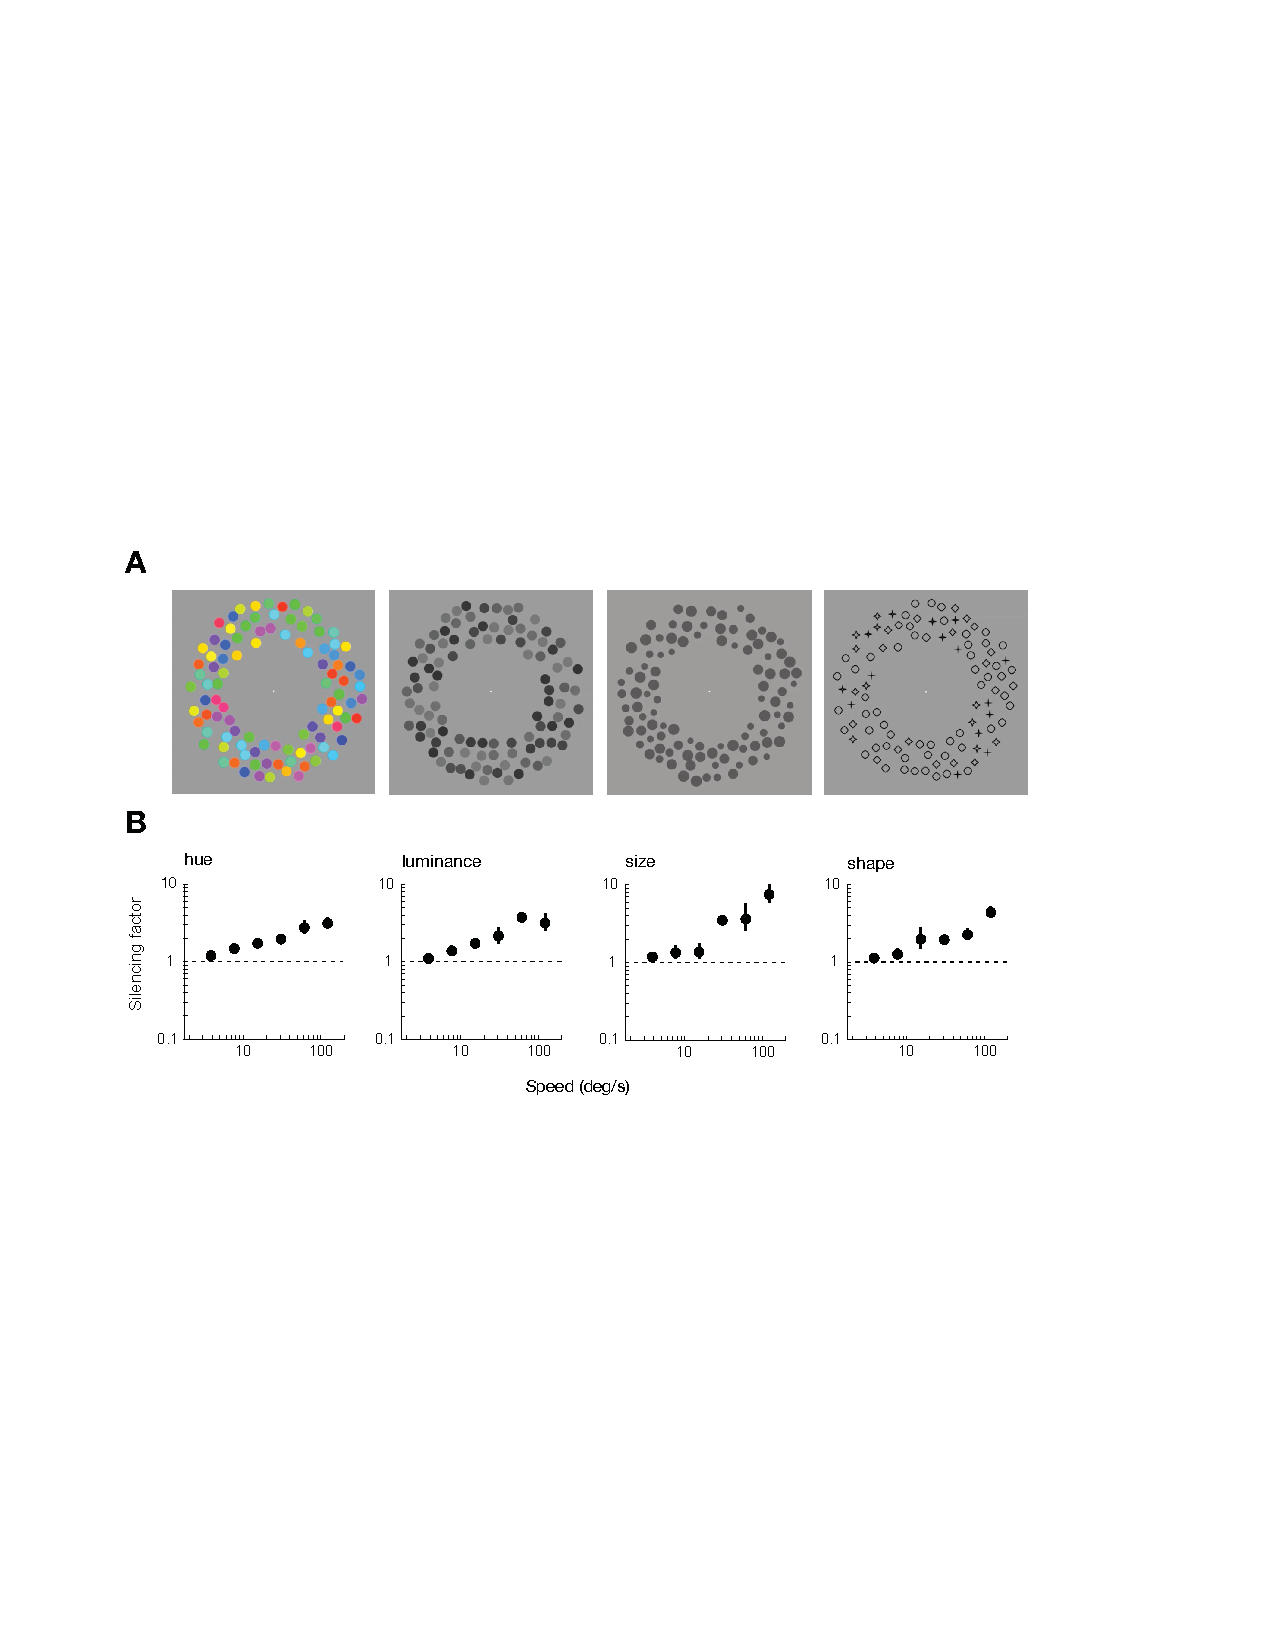
\includegraphics[width=\textwidth]{figures/fig1}
%\caption[Short figure name.]{This is a figure that floats inline and here is its caption.
%\label{fig:myInlineFigure}}
%\end{figure}

% For an example of a full page figure, see Fig.~\ref{fig:myFullPageFigure}.

%% Requires fltpage2 package
%%
% \begin{FPfigure}
% 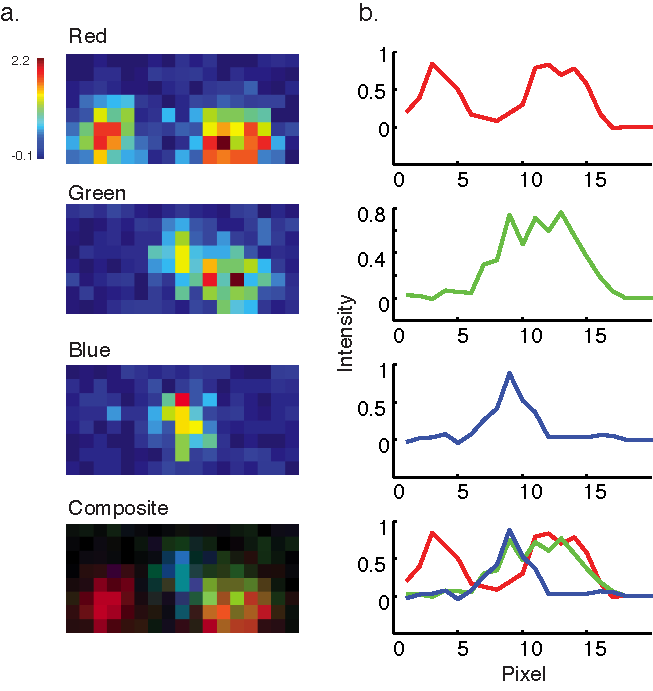
\includegraphics[width=\textwidth]{figures/fullpage}
% \caption[Short figure name.]{This is a full page figure using the FPfigure command. It takes up the whole page and the caption appears on the preceding page. Its useful for large figures. Harvard's rules about full page figures are tricky, but you don't have to worry about it because we took care of it for you. For example, the full figure is supposed to have a title in the same style as the caption but without the actual caption. The caption is supposed to appear alone on the preceding page with no other text. You do't have to worry about any of that. We have modified the fltpage package to make it work. This is a lengthy caption and it clearly would not fit on the same page as the figure. Note that you should only use the FPfigure command in instances where the figure really is too large. If the figure is small enough to fit by the caption than it does not produce the desired effect. Good luck with your thesis. I have to keep writing this to make the caption really long. LaTex is a lot of fun. You will enjoy working with it. Good luck on your post doctoral life! I am looking forward to mine. \label{fig:myFullPageFigure}}
% \end{FPfigure}
% \afterpage{\clearpage}

%\texttt{This is a line of code.}

\newthought{This chapter lays out the design and implementation}, of the system used to generate optimal rule lists. 
We begin by describing each of the three main data structures used to run our algorithm--a prefix trie, a symmetry-aware map, and a queue. 
Then, we 

\subsection{Prefix Trie}
The prefix trie is a custom C++ class which is used as a cache to keep track of rule lists we have already evaluated. 
Each node in the trie contains the metadata associated with that corresponding rule list. 
This metadata includes bookkeeping information such as what child rule lists are feasible as well as information such as the lower bound and prediction for that rule list.
In addition to our BaseNode class, there are two different node types that we use in our algorithm.
Firstly, we implement a CuriousNode class that has an additional field that tracks the curiosity of a given prefix.
The curiosity metric is the one described in Chapter \ref{bounds}.
The curiosity is used to determine the order that prefixes on the queue are explored.
Secondly, we implement a CapturedNode class that extends on the CuriousNode by having an additional field keeping track of the captured vector for that prefix.
This allows us to speed up our incremental computations at the expense of using more memory per node (otherwise we have to recompute this vector every time we have a computation).

\subsection{Queue}
The various node types determine what type of search policy we use to explore the search space.
We use a STL C++ priority queue to hold all of the leaves of the trie that still need to be explored.
We implement a number of different scheduling schemes including BFS, DFS, and a priority queue.
The priority queue can be ordered by curiosity, the objective of a prefix, or the lower bound of a prefix.
We also have a stochastic exploration process that bypasses the use of a queue by walking down the trie, randomly choosing a child each time, until a leaf is chosen to be explored.
We find that ordering by curiosity will often, but not always, lead to a faster runtime than using BFS.

Since we do not have access to the container underlying the queue, we cannot randomly access elements in the queue, even if we have a pointer to the leaf node in the prefix trie.
Thus, we run into a problem where we may delete something in the prefix trie that is currently in the queue, but have no way to update the queue.
We deal with this by lazily deleting nodes from the prefix trie.
This means we mark the node as deleted in the trie, but don't actually delete the physical node until it has been popped off of the queue.
As Fig \ref{fig:queue_gc} shows, this leads to a situation where our logical queue is actually smaller than the physical queue.

\begin{figure}[t!]
\begin{center}
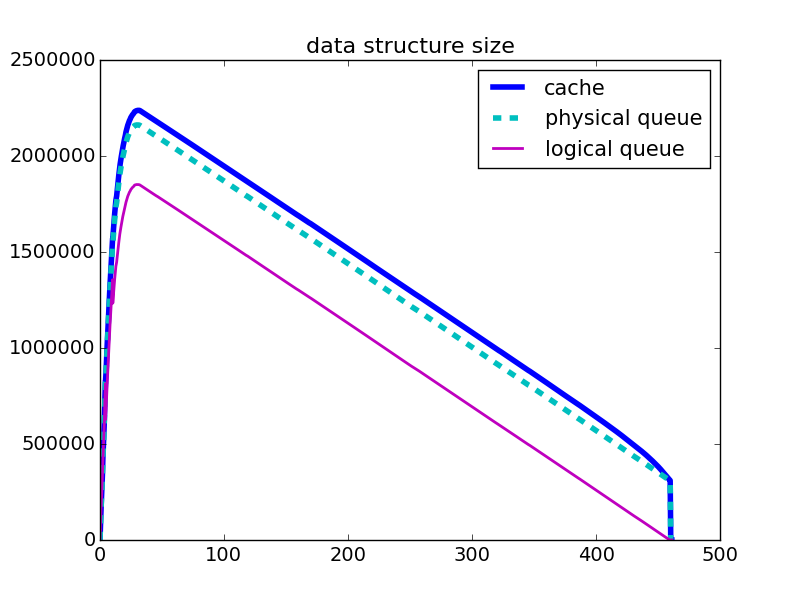
\includegraphics[width=0.65\textwidth]{figs/ela_compas-queue-cache-size-insertions.png}
\end{center}
\caption{Difference between logical cache and physical cache}
\label{fig:queue_gc}
\end{figure}

\subsection{Symmetry-aware map}
We implement the symmetry-aware map as an STL unordered\_map. 
We use this data structure to implement the permutation bound described in \ref{def:perm-bound}.
We have two different versions of the map with different keys that both allow permutations to be compared and pruned.
In both cases, the values contain the actual ordering of the rules that represents the current best prefix for that permutation.
In the first version, keys to the map are represented as the canonical order of rule lists: i.e. the lists 3-2-1 and 2-3-1 both map to 1-2-3.
The second version has keys that represent the captured data points.
Our earlier permutation bound was based off of the fact that different permutations capture the same data, so this type of key will again be equivalent for the rule lists 3-2-1 and 2-3-1.
Representing keys with captured vectors could potentially match more permutations, but requires more memory.
Since most data sets have a large amount of data, the keys representing the canonical ordering are usually more efficient.
In general, for long runs of our algorithm, the permutation map dominates our memory usage.

\subsection{Incremental execution}
Our program executes as follows. 
While there are still leaves of the trie to be explored, we use our scheduling policy to select the next rule list to evaluate.
Then, for every rule that is not already in this rule list, we calculate its lower bound, objective, and other metrics that would occur if the rule were added to the end of the rule list.
If the lower bound is greater than the minimum objective, meaning this new rule list could never be better than one we have already seen, we don't insert the new rule list into the tree or queue.
We next check if there is a better permutation of this rule list in the permutation map and discard the new rule list if it is not better than the rule list we already have in the permutation map.
If our new rule list is better, then we insert it into the permutation map, the tree, and the queue and update the minimum objective if necessary.

Every time we update the minimum objective, we garbage collect on the trie.
We do this by traversing from the root the all of the leaves, deleting any subtrees of nodes with a lower bound that is larger than the minimum objective.
In addition, if we encounter a node with no children, we prune upwards--deleting that node and recursively traversing the tree towards the root, deleting any childless nodes.
This garbage collection allows us to limit the memory usage of the trie, though garbage collection is not triggered too often.

\begin{algorithm}[t!]
  \caption{Branch-and-bound for learning rule lists}
\label{alg:branch-and-bound}
\begin{algorithmic}
\normalsize
\State $obj \gets 0$
\State $bestRL \gets NULL$
\State $T \gets initializeTree()$
\State $Q \gets queue(\,[T.root()\,])$
\State $P \gets map(\{\})$
\While {$Q$ not empty}
	\State $node \gets Q.pop()$
	\State $oldObj \gets T.min\_objective()$
	\State $incremental(node, T, Q, P)$ \Comment{Evaluate all of node's children}
	\If {$T.min\_objective() < oldObj$}
		\State $T.garbageCollect()$
	\EndIf
\EndWhile


\end{algorithmic}
\end{algorithm}

\begin{algorithm}[t!]
  \caption{Incremental evaluation of a prefix}
\label{alg:incremental}
\begin{algorithmic}
\normalsize
\State \textbf{Input:} Node to be evaluated~$parent$,
prefix tree~$T$,
queue~$Q$,
symmetry-aware map~$P$
\State \textbf{Output:} newObj~Best objective in the tree\\
\State $prefix \gets parent$.prefix()
\State $t \gets \lambda *$ nsamples \Comment{This forms the threshold for our support bounds}
\For {$rule \notin prefix$}
	\State $rlist \gets prefix$.append($rule$)
	\State $cap \gets parent$.not\_captured() $\wedge rule$.not\_captured()
	\If {$|cap| < t$} \Comment{Minimum support bound}
		\State continue
	\EndIf
	\State $cap\_0 \gets cap \wedge T->label_0$ \Comment{Record how many zeros the new rule captures}
	\State $cap\_correct \gets max\{|captured\_zeros|, |captured| - |captured\_zeros|\}$
	\If {$|captured\_correct| < threshold$} \Comment{Minimum correct support bound}
		\State continue
	\EndIf
	\State $lower\_bound = parent->lower\_bound - parent->minority + |captured| - |captured_correct| / nsamples + c$
	\If {$lower_bound  >= T->min\_objective()$} \Comment{Objective bound}
		\State continue
	\EndIf
	\If {$objective < T->min\_objective()$} \Comment{Update minimum objective}
		\State continue
	\EndIf
	\If{$lower\_bound + c >= T->min\_objective()$} \Comment{Lookahead bound}
		\State continue
	\EndIf
	\State $n \gets P->insert(rlist)$ \Comment{Symmetry-aware map handles permutation bound for us}
	\If {$n$}
		\State $T->insert(n)$
		\State $Q->push(n)$
	\EndIf
\EndFor
\end{algorithmic}
\end{algorithm}

\subsection{Memory tracking}
We track memory through the use of C++11 custom allocators.
Our allocators essentially just wrap malloc and then log where the allocation is coming from--the trie, the map, or the queue.
We validated the accuracy of this memory tracking by running the program under Valgrind's massif heap profiler tool and comparing the outputs.
Outputs were within a few hundred bytes, so we concluded that our memory tracking was successful.
This allowed us to write out our memory usage per data structure without incurring the large overhead of Valgrind.